\section{Stockholm --- Stockholm Congestion Tax}

\subsection{History}

Discussion of downtown pricing in Stockholm started in the early 1980s, when the local Social Democrats party proposed that cars entering downtown Stockholm be required to display a monthly pass---good for either transit or driving---in their windshields \citep{GullbergIsaksson2009,Arnott2005}. In 1989, the City of Stockholm formulated plans for this so-called ``car card'' proposal as well as an electronic cordon pricing system \citet[p. 90]{Hau1992} for details; but since road pricing was deemed to be a ``tax'' rather than a ``charge,'' Swedish law required that the national parliament approve the scheme. In Autumn 1990, although the local Social Democrats had proposed it, the Social Democrats who controlled the parliament wound up blocking pricing for political reasons \citep{Ahlstrand2001}. 

Meanwhile, recognizing that congestion in Stockholm had become serious, the national government convened Stockholm's political parties to negotiate an infrastructure package. The resulting agreement, finalized in 1992 and called the ``Dennis Package,''  consisted of \$6.1 billion in infrastructure projects designed to keep cars out of downtown Stockholm (see \citet[pp. 39-40]{Gomez-Ibanez1994} and \citet[p. 92]{Hau1992}). About 45\% of the money was slated for public transport, and the rest for large road projects: a bypass about 10km West of the City and a ring road around central Stockholm. To pay for the scheme, electronic tolls would be placed on the western bypass and along the cordon outside the ring road, so as to charge all traffic into Stockholm. However, in 1997 government cancelled the Dennis Package due, as before, to complex political maneuverings \citep{Ahlstrand2001,GullbergIsaksson2009}. Still, despite this failure, the Dennis Package had introduced a very specific road pricing plan into road pricing into Swedish politics and gained the attention of the country's environmental movement \citep[p.3]{Eliasson2014b}.

In 2000, the Swedish parliament set up a ``Stockholm Commission'' to  prioritize infrastructure projects for Stockholm \citep{Eliasson2009b}. To find funding, in March 2002 the government asked it to come up with with new plans for road pricing. As it happened, 2002 was also an election year in Sweden, and the Moderate Party (Sweden's mainstream conservative party) in Stockholm used the renewed discussion of pricing---a divisive issue---to win some voters from their rivals, the Social Democrats. In response, the Social Democrat candidate for Mayor of Stockholm, Anna Billstr\"om, announced on television: ``My message to the voters of Stockholm is that there will be no road charging during our next term of office'' \citep{GullbergIsaksson2009}.

After the September 2002 election, the Social Democrats and their allies, the Left Party, came up just short of a majority both nationally and in Stockholm. Seizing the opportunity, the environmentalist Green Party agreed to join the coallition in exchange for a full-scale trial of pricing in Stockholm. The Social Democrats' acceptance of this offer prompted an outcry over the new mayor Billstr\"om's broken pledge, and opponents demanded that the decision of whether to instate pricing permanently be made via referendum. Seeking to defuse the situation, the government agreed a referendum would follow the trial's conclusion and appear on the September 2006 election ballot.

The trial was initially meant to last several years, but political and legal complications---especially fighting over whether the tolls would be a local or national measure---delayed the start until January 3, 2006. The trial ended on July 31, 2006. Prior to the trial, media coverage of the trial was very negative, and polls showed strong opposition. But once the trial began, public opinion shifted quickly in favor due to very visible congestion reductions. At the September 2006 elections, 53\% of Stockholm residents voted to make the scheme permanent, but the Social Democrats/Green/Left coalition lost control of the government at all levels to a center-right alliance composed of parties who opposed pricing. Thus, for a moment it was unclear whether the new government would respect the referendum results, but in the end the government agreed to do so after negotiating a \euro 10 billion infrastructure package, whereby toll revenues were matched by national funds to build new roads around Stockholm (to the chagrin of environmentalists). The scheme was reactivated on XXX and continues in operation today.

\subsection{Design}

The Stockholm Congestion Tax is a time-variable toll on weekday trips in either direction across a cordon around central Stockholm. Crossings in both directions pay the same toll. See Figure \ref{fig:stockholm-map} for a map of the approximately 35 km$^{2}$ charging zone. Note from the map that water boundaries require only 18 access points to establish the cordon. Vehicles are charged each time they pass under gantries, which function in sets of three: when a laser on the middle gantry detects a vehicle passing below, cameras mounted on the first and third photograph the front and rear plates \citep{FAQ2015}. Foreign, emergency, diplomatic, alternative-fuel and foreign-registered vehicles were exempt at first, but the alternative-fuel exemption was ended in August 2012.

\begin{figure}
\includegraphics[width=5in]{../img/stockholm-map.png}
\caption{Stockholm Congestion Tax, access points in red. \citep{transportstyrelsen2015}}
\label{fig:stockholm-map}
\end{figure}

INCLUDE XXX: Lindigo exemption, technology


\begin{figure}
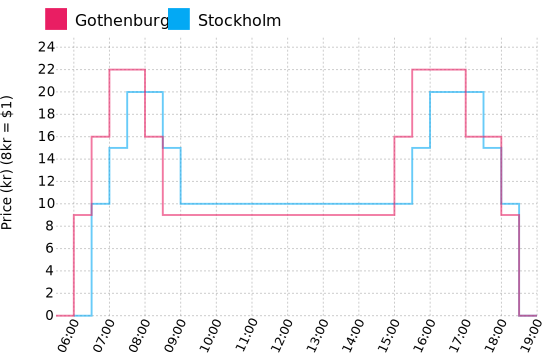
\includegraphics[width=5in]{../img/sweden-prices.png}
\caption{Sweden price structure \citep{transportstyrelsen2015}}
\label{fig:sweden-schedules}
\end{figure}

\subsection{Results}

The Tax has cut both traffic flow and travel times. Traversals of the cordon have fallen by 20-21\%. This figure was in excess of the forecast 16\% fall, due to the fact off-peak travel fell by almost the same amount (21\%) as peak travel (20\%) \citep{Eliasson2013}. Models had predicted off-peak travel would fall only 14\% due to lower mid-day charges. The fall in person-trips was similar for commuters (24\%) and discretionary travelers (22\%), but the two groups adapted differently: commuters who stopped driving switched to public transit, while discretionary travelers cancelled or rerouted their trips \citep{FranklinEtAl2010}. \citet{Eliasson2013} estimate that the Tax raised public transit ridership 4-5\%, or 8-10 thousand riders per day, and that vehicle-kilometers-traveled within the zone fell 10-15 percent. \citet{Karlstrom2009} find only weak evidence of departure time rescheduling.

\subsection{Finances}
Costs due to delays 600 MSEK \citet[p. 843]{GullbergIsaksson2009}.

Congestion Tax not so different than the gasoline tax, which is collected and then redistributed.